% ENEL 617 Radio Frequency Integrated Circuits Project Report
% Pouyan Keshavarzian
% Winter 2017
% Master's of Science in Electrical Engineering studies

%-------------------------------------------------------------------------------
% DOC SETUP
\documentclass{article}                                                         % document type
\usepackage[margin=0.7in]{geometry}                                             % Set margins
\usepackage{hyperref}                                                           % Enables typesetting of hyperlinks
\usepackage{float}                                                              % Required to keep images where they are put
\usepackage[dvipsnames]{xcolor}                                                 % More colors!
\usepackage{graphicx}                                                           % Required for the inclusion of images
\usepackage{listings}                                                           % Required for the inclusion of source code
\usepackage{mathtools}                                                          % Math looks pretty. Main backbone is amsmath
\usepackage{enumitem}                                                           % Required to use different characters for enumerated lists
\usepackage{multirow}                                                           % Create tabular cells spanning multiple rows
\usepackage[toc]{glossaries}                                                    % Create glossary
\usepackage[titletoc]{appendix}                                                 % Create Appendix
\usepackage{wrapfig}                                                            % Needed for wrapping text around a figure
\usepackage{subfig}                                                          % Subfigures
%\usepackage[]{mcode}                                                           % Matlab code
\setlength\parindent{0pt}                                                       % Removes all indentation from paragraphs
\providecommand{\e}[1]{\ensuremath{\times 10^{#1}}}                             % Use scientific notation
%\usepackage{times}                                                             % Uncomment to use the Times New Roman font
\usepackage{pdfpages}                                                           % Simplifies inclusion of external multi-page pdfs into document
\loadglsentries[main]{glossary}                                                 % Glossary
\makeglossaries
\usepackage[backend=bibtex, firstinits=false, style=numeric-comp]{biblatex}
\addbibresource{Bibliog.bib}
\usepackage{verbatim}                                                           % Does things verbatim?? For example \verbatiminput{appendices/GuitarTunerApp.mc}. Also adds \begin{comment}. Also reporduces text verbatum
\usepackage{pdflscape}                                                          % For landscape pages

%-------------------------------------------------------------------------------
%----------------------------------------------------------------------------------------
%	DOCUMENT TITLE PAGE
%----------------------------------------------------------------------------------------
\title{\textsc{\textbf{ENEL 617 WINTER 2017 PROJECT REPORT}}} % Title
\author{\textsc{Millimeter-Wave Double Balanced Gilbert Mixer}
\\ \textsc{Pouyan Keshavarzian}}
\date{\today} % Date for the reports
\begin{document}
\maketitle % Insert the title, author and date
\newpage
%----------------------------------------------------------------------------------------
%	Table of Contents and Figures
%----------------------------------------------------------------------------------------
% Add tables and lists as required
\tableofcontents
\listoffigures
\listoftables
%-------------------------------------------------------------------------------
\newpage
%----------------------------------------------------------------------------------------
%	GLOSSARY
%----------------------------------------------------------------------------------------
%\section{Glossary}
%\printglossary[title=Terms Acronyms and Abbreviations]
%\newpage
%----------------------------------------------------------------------------------------
%	SECTION
%----------------------------------------------------------------------------------------
\section{PROJECT MOTIVATION}
A double balanced mixer that would be used as part of a  BPSK Modulator circuit
to generate a spread spectrum radar waveform in the automotive frequency band (77-81 GHz) is presented. A similar modulator
that uses a double-balanced mixer is described in \cite{schleicher2010biphase}. The original design benchmarks for this mixer
and the achieved final results are outlined in Table ~\ref{table:goalsnresults}.\vspace{3mm}
\vspace{3mm}
\begin{table}[H]
\centering
 \begin{tabular}{ | c | c | c |}
   \hline
    \textbf{Parameter} & \textbf{Original Targets} & \textbf{Achieved}  \\
    \hline
    \hline
    Supply Voltage & 1.8V & 0.85V \\
    \hline
    Power Consumption & 5mW & $\approx$ \textbf{\textcolor{OliveGreen}{4.8mW}}\\
    \hline
    Gain (dB)   & 5 & $\approx$ \textbf{\textcolor{Red}{-13 dB}} \\
    \hline
    Input Match  & 50$\Omega$ & \textbf{\textcolor{OliveGreen}{45.5 + j0.1$\Omega$}} \\
    \hline
    Output Match & 730$\Omega$ & \textbf{\textcolor{Orange}{48.9 + j0.1$\Omega$}}\\
    \hline
    NF & 10dB & $\approx$ \textbf{\textcolor{Red}{16 dB}}\\
    \hline
    P1dB & -- & $\approx$ 1.5dB  \\
    \hline
    IP3 & -- & $\approx$ 9.5dB  \\
    \hline
  \end{tabular}
  \caption{Mixer Design Targets and Achieved}
  \label{table:goalsnresults}
\end{table}
The original values were generated based on a few simple simulations/calculations and a power budget provided by Dr. Belostotski. The
power budget was the control variable that is set as an absolute requirement.  Once the Id-gm
characteristics were understood from simulation, the gain estimate was calculated using the following equation.
\begin{equation}
  \label{eq:idealgain}
  G=\dfrac{2}{\pi}\dfrac{R_L}{R_s + \dfrac{1}{g_m}};
\end{equation}
The exact values including plots for the final results will be clearly outlined. Furthermore, deviations from original to achieved results
will be described in detail. A different design topology was used in the final design than in the original biased circuit used to calculate
the conversion gain. Some targets (such as output impedance) were changed intentionally (for practical purposes) while other values
were adjusted based on non-ideal aspects of the circuit.\vspace{3mm}
A derivation of conversion gain will be provided in the theory of operation section. A suitable value of $R_L$ was chosen
based on biasing and achieving high gain.
The interest in this particular-type of radar stems from spread-spectrum technology's built in interference rejection, which
is an indispensable feature for automotive radar. This type of radar has recently been demonstrated in
SiGe technology \cite{trotta200779ghz, ng2014fully}. 65nm technology is chosen because the Figure of Merit, $f_T \approx 160GHz $, making it suitable for
this millimeter-wave application.\\

\textbf{Note} that simulations are redone in Matlab for ease of viewing. Original plots from Cadence are available in the Appendix.

\newpage
\subsection{Radar Theory of Operation}

\begin{wrapfigure}{r}{0.5\textwidth}
  \begin{center}
    \includegraphics[width=0.4\textwidth] {Figures/radarblock.png}
    \caption{Radar Transceiver Block Diagram}
    \label{fig:radartrans}
  \end{center}
\end{wrapfigure}
To demonstrate how this mixer could be used in a practical application, the theory of the type of radar is discussed.
A simplified block diagram of an example spread spectrum ranging system is shown in Figure ~\ref{fig:radartrans}.
The BPSK modulator is used to spread the carrier with a pseudorandom code. The parameters of the code, which govern
the LO mixing frequency, are designed to provide an adequate range resolution within the context of automotive radar.
The achievable range resolution of the radar system is related to the chip rate (mixer LO) of the code through
Equation ~\ref{eq:rangeres}. This is fairly intuitive as the frequency of this signal determines the time-resolution,
thereby determining the resolution of range. \\

\begin{equation}
  \label{eq:rangeres}
  d_{min} \leq \dfrac{c}{2f_c}
\end{equation}

Therefore to achieve a $10cm$ range resolution a chip rate of $1.5 GHz$ is chosen. The rest of the code can be designed by
choosing the appropriate length. \\
\begin{equation}
  \label{eq:codelength}
  T_{p} = \dfrac{N}{f_c}
\end{equation}
and then achievable unambiguous range of the radar becomes
\begin{equation}
  \label{eq:maxrange}
  d_{max} \leq \dfrac{c}{2T_p}
\end{equation}
Since the code is pseudorandom, the LO frequency could be any integer division of $1.5GHz$ i.e $0.75GHz, 0.5GHz$ etc.
For the purposes of design we will simulate with just a $1.5GHz$ signal to demonstrate the maximum bandwidth of operation.
\newpage
\section{Mixer Theory of Operation}
\subsection{Basic Principle}

The Gilbert Cell is a linear time-varying circuit. The concept behind this circuit is intuitive. The RF transistors act as
amplifiers which change the input voltage to a current. The LO ports act as switches that commutate the output.
This creates the time-domain multiplication function. Figure \ref{fig:simpmix} demonstrates this concept.
\begin{figure}[H]
  \centering
  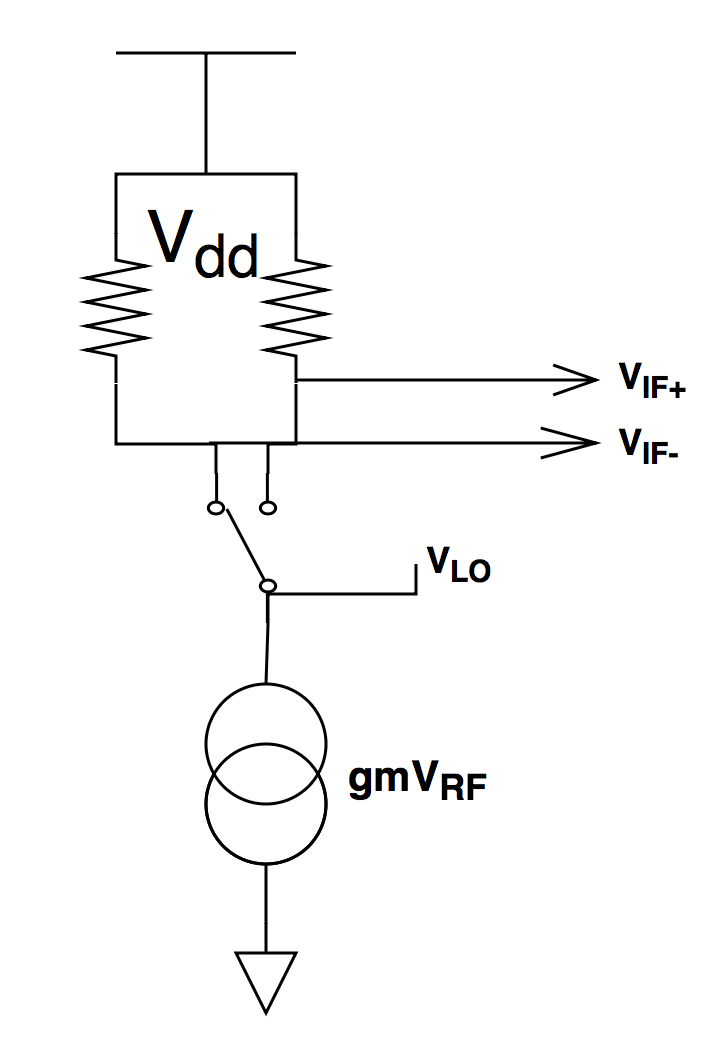
\includegraphics[width=0.2\textwidth] {Figures/gilbertSimple}
  \caption{Mixer Theory}
    \label{fig:simpmix}
\end{figure}

Since the Gilbert Cell is a double balanced, i.e. both RF and LO inputs are differential, the signals get subtracted out at IF. Therefore,
there should be very little of the RF and LO frequencies present at the output.
\subsection{Conversion Gain}
As previously mentioned, the LO differential pairs essentially act as switches thereby allowing current to flow through resistors $R_1$
and $R_2$.
\begin{equation}
  \label{eq:I1}
  I_1 = I_{RF}F_{T}
\end{equation}
and
\begin{equation}
  \label{eq:I2}
  I_2 = I_{RF}F_{T}(t-\dfrac{T_{LO}}{2})
\end{equation}

where $F_{T}$ is the square wave with period $T_{LO}$. The voltage at IF is equal to:

\begin{equation}
  \label{eq:VIF}
  V_{IF} = V_{DD} - I_1R_L - (V_{DD}-I_2R_L)
\end{equation}
\begin{equation}
  \label{eq:VIFt}
  V_{IF}(t) = I_{RF}(t) R_L [F_{T}(t-\dfrac{T_{LO}}{2})-F_{T}]
\end{equation}

\vspace{5mm}Since $F_T$ is a square wave it can be seen that multiplying by $F_{T}(t-\dfrac{T_{LO}}{2})-F_{T}$
is the same as multiplying by a square\vspace{3mm} wave with amplitudes ranging from 1 to -1. Using the Fourier
expansion of this square wave we get

\begin{equation}
  \label{eq:VIFt2}
  V_{IF}(t) = I_{RF}(t)R_L[\dfrac{4}{\pi}cos(\omega_{LO}t)...]
\end{equation}
\begin{equation}
  \label{eq:VIFt3}
  V_{IF}(t) = \dfrac{2}{\pi}g_{m1}R_LV_{RF}cos((\omega_{RF}-\omega_{LO})t)
\end{equation}
The peak conversion gain is then:
\begin{equation}
  \label{eq:Vgain}
  \dfrac{V_{IF,p}}{V_{RF,p}} = \dfrac{2}{\pi}g_{m1}R_L
\end{equation}
\vspace{3mm}If you have a source resistor then the gain drops proportionally, arriving at Equation ~\ref{eq:idealgain}.

\subsection{Biasing}
Biasing was done to maximize $g_m$ for gain while remaining under the power budget. With a $V_{dd}$ of 0.85V
the total bias current can be calculated:
\begin{equation}
  \label{eq:biascurrent}
  I_{DC} = \dfrac{5mW}{0.85V} = 5.9mA
\end{equation}

\subsection{RF Port Matching}
Originally the RF port was going to be matched with a $50 \Omega $ source resistor. After understanding that the
matching of this circuit could be designed using the same methodology as a source-degenerated LNA topology and also encountering
voltage headroom problems, it became apparent that using source and gate inductors to match was the best option. The source inductor is
used to match to $50\Omega$ and the source and gate inductors combined are used to resonate out $C_{gs}$ (and in the case of high frequency
many other parasitics).
\begin{equation}
  \label{eq:InputRes}
  50 \Omega = \omega_TLs
\end{equation}
\begin{equation}
  \label{eq:GateInd}
  \dfrac{1}{w(sC_{gs}+C_{others})} = \omega(L_s+L_g)
\end{equation}

\vspace{3mm}For 65nm technology $\omega_T \approx 2\pi \times 160GHz$ \cite{Razavi:2011:RM:2132691}.
This method of calculating input impedance is derived by ignoring the common gate transistor,
other capacitances and $g_{ds}$ of the common source (RF) transistor. \\

This method is greatly oversimplified for an 80GHz circuit, seeing as there are parasitic capacitances and a finite output resistance.
Therefore an attempt is made to create an improved input impedance model. This is discussed in Section ~\ref{sec:matching}

\subsection{IF Port Matching}
The output matching circuit was originally conceived to be resistive. Again, after learning more about the method of designing this circuit and
the limitations involved, it became clear that an LC tank was required. Therefore the tank was designed to resonate at the desired frequency and the resistive
load chosen to meet the output impedance requirement. Furthermore to get an output impedance as high as $700\Omega$ a very large resistance would be required. This
is because $g_{ds}$, which is in parallel with the load resistor, is of a very similar magnitude.  As will be discussed in the simulation section, none of these values were as expected
because of all the transistor parameters not taken into account.

\subsection{Noise}
Analyzing noise in active double-balanced mixers is complicated. The same methods studied for LNA noise optimization can be implemented however
there are other variables that must be considered. As will be discussed in later sections, mixing with a sin wave (as is done in simulation) will increase noise figure.
Furthermore, with this design there are quite a few resistors and no noise optimization is actually considered. Typical SSB of between 10-15dB is
to be expected for this type of mixer therefore the achieved value seems acceptable.

\subsection{Linearity}
This design was largely done without taking linearity into consideration. The source inductor naturally provides some
improvements because of negative feedback.

\newpage
\begin{landscape}
\section{Design Variations and Final Circuit Schematic}
\subsection{Circuit Schematic}

\begin{figure}[H]
  \centering
  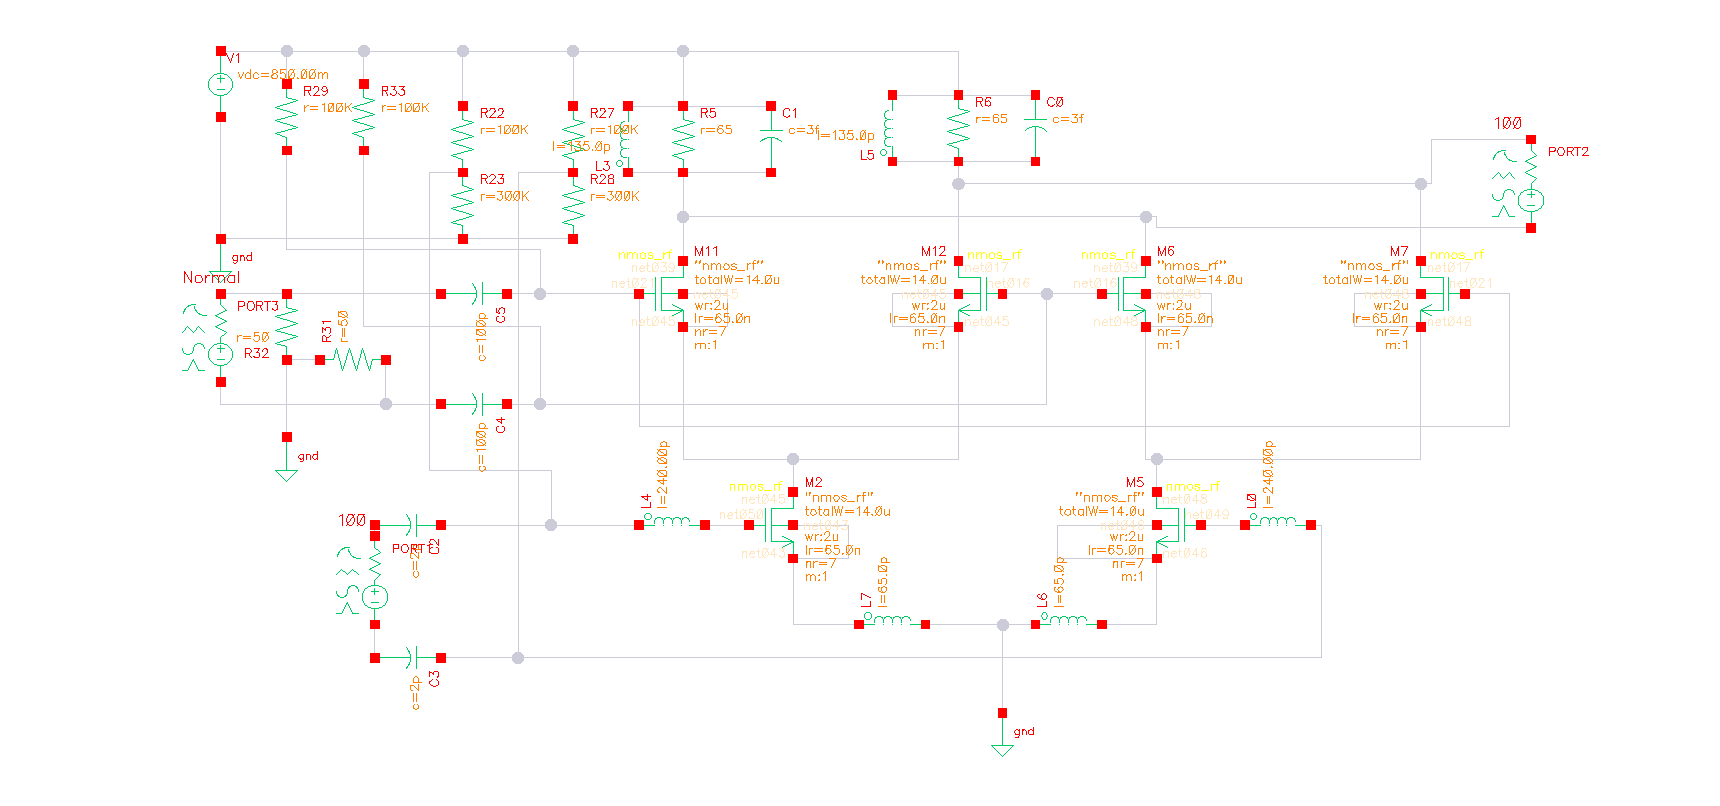
\includegraphics[width=1.5\textwidth] {Figures/Circuit.png}
  \caption{Final Design}
    \label{fig:finalschem}
\end{figure}
\end{landscape}
\newpage

\begin{table}[H]
\centering
 \begin{tabular}{ | c | c |}
   \hline
    \textbf{Component} & \textbf{Final Values}   \\
    \hline
    \hline
    $W$, Transistor Width & $14 \mu H$ \\
    \hline
    $L$, Transistor Length & $65nm$ \\
    \hline
    $L_s$, Source Inductor & $65pH$ \\
    \hline
    $L_g$, Gate Inductor & $240pH$ \\
    \hline
    $R_L$, Source Resistance & $65\Omega$ \\
    \hline
    $L_T$, Tank Inductor & $130pH$ \\
    \hline
    $C_T$, Tank Capacitor & $3pF$ \\
    \hline
    $C_c$, DC block/AC Short Cap & $100pF$ \\
    \hline
    $V_{bias,LO}$ & 0.85V \\
    \hline
    $V_{bias,RF}$ & 0.64V \\
    \hline
  \end{tabular}
  \caption{Mixer Final Component Values}
  \label{table:finalvals}
\end{table}
\subsection{Overall Design Strategy Variation}

At first the circuit was designed with a 1.8V power supply and a cascode type current mirror for biasing.
However, this topology was causing many problems. First of all, the node at the current mirror
had to maintain at least $\approx$ 0.4V for the current mirror to function properly. Voltage headroom and being able to design for a $V_{od}$
of $\approx$ 0.1V while also staying under the power budget of 5mW became an issue. Since, in this configuration,
the current had to be kept low $V_{ds}$ was high, further aggravating the voltage headroom issue. Furthermore operating at
1.8V is not advised since that is the breakdown of 65nm technology.\\

\vspace{3mm}
After (a couple weeks of) using that topology, it became apparent that the best option was to scrap the current mirror. Dropping the
supply voltage also allowed for more current, thereby reducing $V_{ds}$. An LC
tank was also added to increase voltage headroom and it later became apparent that those components would
also be required for output matching because of all the parasitics present.
This then allowed for an increase in transistor width, which in turn increases the transconductance and thereby the gain.
Originally with the power restriction, the largest achievable transconductance was $\approx 5mS$ and the overdrive voltage
was $\approx 50mV$. After the topology change it was much easier to achieve an overdrive voltage of $\approx 100mV$ and $g_m
\approx 14mS$. All final values are shown in Table ~\ref{table:parameters}.\\
\subsection{Output Impedance Change}

At first, an output resistance of 730$\Omega$ was chosen to achieve the target gain of approximately 5dB based on calculations using
Equation ~\ref{eq:idealgain}.
This was not a very well thought out choice. It would be unusual to have such a high output impedance since the practical
implementation of this would need to interface with other circuits (namely a PA). Therefore the target was reduced
to 50$\Omega$. The reduction in gain from this change was somewhat compensated by the fact that $g_m$ is now improved.

\subsection{Conversion Gain Change}
With the other changes outlined, it is now pertinent to recalculate conversion gain. Using Equation ~\ref{eq:Vgain} and using
values of $g_m = 14mS$ and $R_L = 50 ohm$

\begin{equation}
  \label{eq:gaintargetnew}
  G = 20\log(\dfrac{2}{\pi}g_mR_L) \approx -7dB
\end{equation}

\vspace{3mm}\textbf{Note} that this calculation is done with a square wave which maximizes
conversion gain. During simulation, mixing is done with a sine wave and so there is a period of time
where both transistors in the differential pair are on. This reduces gain and increases noise figure.
We would then expect the simulated gain to be below this calculation. In fact, the gain equation is reduced
proportionally to $\Delta T$, the time of overlapping drain current waveforms in the switching pair.

\begin{equation}
  \label{eq:gaintargetnew}
  G = 2\pi g_m R_L (1 -\dfrac{2\Delta T}{T_{LO}})
\end{equation}

\newpage
\section{Simulated Results}
\subsection{Transistor Biasing and Power Consumption}
\begin{table}[H]
  \small
  \centering
  \caption{Final Values For DC Analysis}
  \subfloat[RF Transistors]{%
    \hspace{.5cm}%
    \begin{tabular}{|c|c|}
      \hline
      \textbf{Parameter} & \textbf{Value} \\
      \hline
      \hline
      $I_D$ &  2.819mA \\
      \hline
      $C_{gs}$ &  9.468fF \\
      \hline
      $C_{gd}$ &  3.613fF \\
      \hline
      $g_m$ &  14.94mA/V \\
      \hline
      $g_{ds}$ &  2.94mA/V \\
      \hline
      $V_{ds}$ &  331mV \\
      \hline
      $V_{gs}$ &  646mV \\
      \hline
      $V_{th}$ &  414mV \\
      \hline
      \hline
    \end{tabular}%
    \hspace{.5cm}%
  }\hspace{1cm}
  \subfloat[LO Transistors]{%
    \hspace{.5cm}%
    \begin{tabular}{|c|c|}
      \hline
      \textbf{Parameter} & \textbf{Value} \\
      \hline
      \hline
      $I_D$ &  1.409mA \\
      \hline
      $C_{gs}$ &  8.754fF \\
      \hline
      $C_{gd}$ &  3.216fF \\
      \hline
      $g_m$ &  12.18mA/V \\
      \hline
      $g_{ds}$ &  1.38mA/V \\
      \hline
      $V_{ds}$ &  510mV \\
      \hline
      $V_{gs}$ &  511mV \\
      \hline
      $V_{th}$ &  402mV \\
      \hline
      \hline
    \end{tabular}%
    \hspace{.5cm}%
  }
\label{table:parameters}
\end{table}

Overdrive voltage for LO transistors was lower than RF transistors. This is because it was important
that the LO transistors would fall into triode and cutoff with the corresponding LO swing. The overdrive
voltage for the RF transistors was designed high to get high transconductance while still remaining in saturation.
The total current $I_{DC} = 2.819mA \times 2 = 5.638mA$ gives a power consumption of $P = 5.638mA \times 0.85V = 4.8mW$


\subsection{Conversion Gain}
\begin{figure}[H]
  \centering
  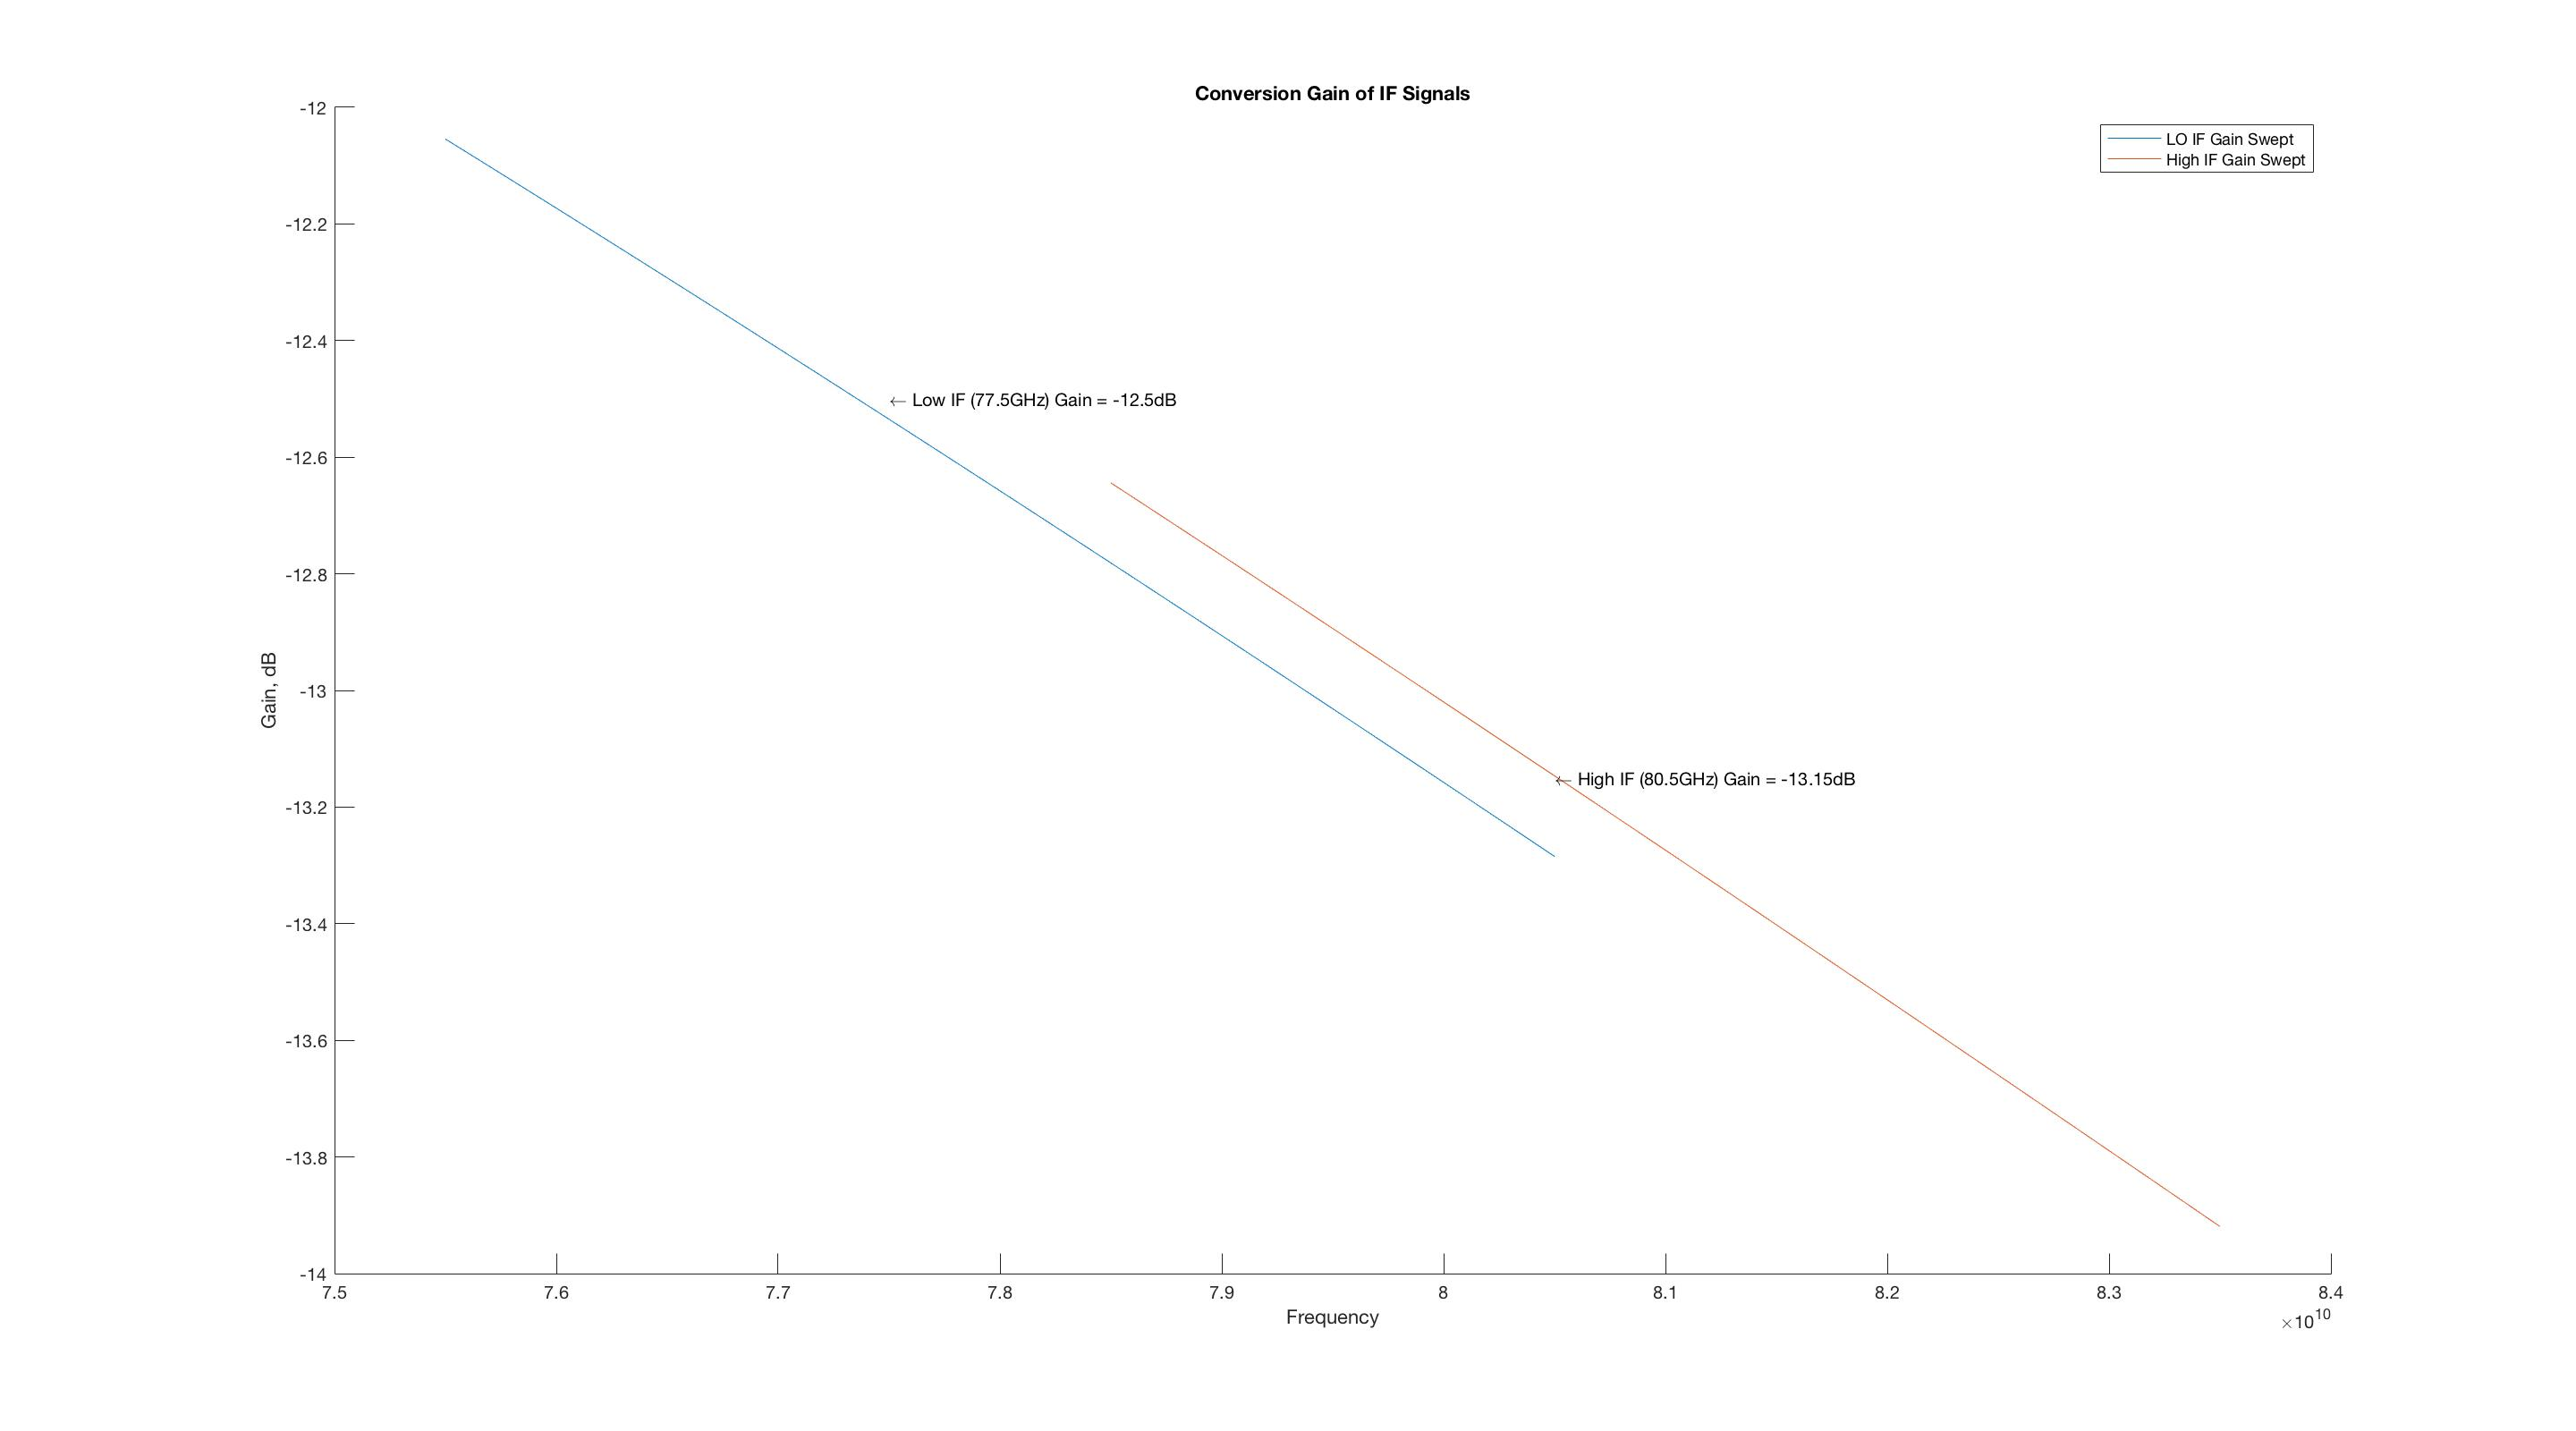
\includegraphics[width=0.95\textwidth] {Plots/Gain.jpg}
  \caption{Swept Gain for Lo/Hi IF}
    \label{fig:matgain}
\end{figure}
The achieved conversion gain (once matched) is slightly lower then the calculated value based on Equation
~\ref{eq:gaintargetnew} as expected because of the slow switching of the LO transistors.\\
\textbf{Note} RMS spectrum is shown in the Appendix.
\subsection{Input and Output Matching}\label{sec:matching}
\subsubsection{Theory}
As previously discussed, the source degenerated topology input impedance is defined by the
simple circuit seen below.

\begin{figure}[H]
  \centering
  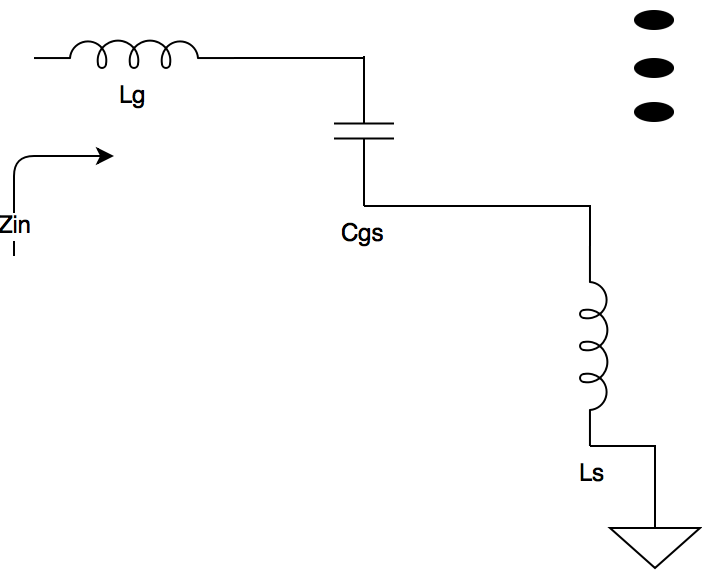
\includegraphics[width=0.3\textwidth] {Figures/zin}
  \caption{Simplified Input Impedance}
    \label{fig:zinSimple}
\end{figure}

From this model, Initial values of $Ls = 50pH$ and $L_g = 390pH$ are picked based on the simulated bias value of $C_{gs}$.
As a side exercise, an attempt at producing an analytical improved impedance model for the cascode which considers $g_{ds}$
and $C_{gd}$ of both transistors was done and is shown in Appendix ~\ref{app:imp}.
This model was then used in Matlab with chosen values of $L_s$ in an attempt to get an optimized answer as opposed to the oversimplified number produced
by the source degenerated cadcode LNA model. In theory, once values of $L_s$ were analyzed then a more accurate value of $L_g$ could
also be chosen based on the remaining reactance. However the calculations produced by this model and Matlab did not seem to be any closer
than the original model. In the end, changing the values based on simulation seemed to be the only reliable method.\\

After iterative simulation the values of $Ls = 65pH$ and $L_g = 240pH$ were picked as shown in Table ~\ref{table:finalvals}.
These are relatively close to the original guess. It would be expected that the final gate inductance value would be lower than
the initial guess because $C_{others}$ i.e. the parasitics would reduce the value of Equation ~\ref{eq:GateInd}.

\subsubsection{Results}
Good matching is achieved as shown in Figure ~\ref{fig:matS11}. Several iterations of plotting the impedance on the Smith Chart tool
in Cadence was used to achieve the required input match. The values for the output components are quite different then originally expected. The resistance is
slightly higher (65 as opposed to 50). This can be explained by noting that $g_{ds}$ of the LO transistor is in parallel with $R_L$ therefore a
higher Resistor value is needed to achieve $50 \Omega$. The tank was originally designed using
$$ \omega = \dfrac{1}{\sqrt{LC}}$$

with a chosen value of C = 3pF to start the Inductor value comes out to be approximately 1.3nH. However, after simulated the final value of
the inductor chose was about 1/10th that value (Note Dr. Belostotski ignore the conversation we had about it being higher... I got it backwards). This
makes sense because of all the parasitic capacitances that are present. The -10dB bandwidth for both S11 and S22 extends past the entire operating band.
\begin{figure}[H]
  \centering
  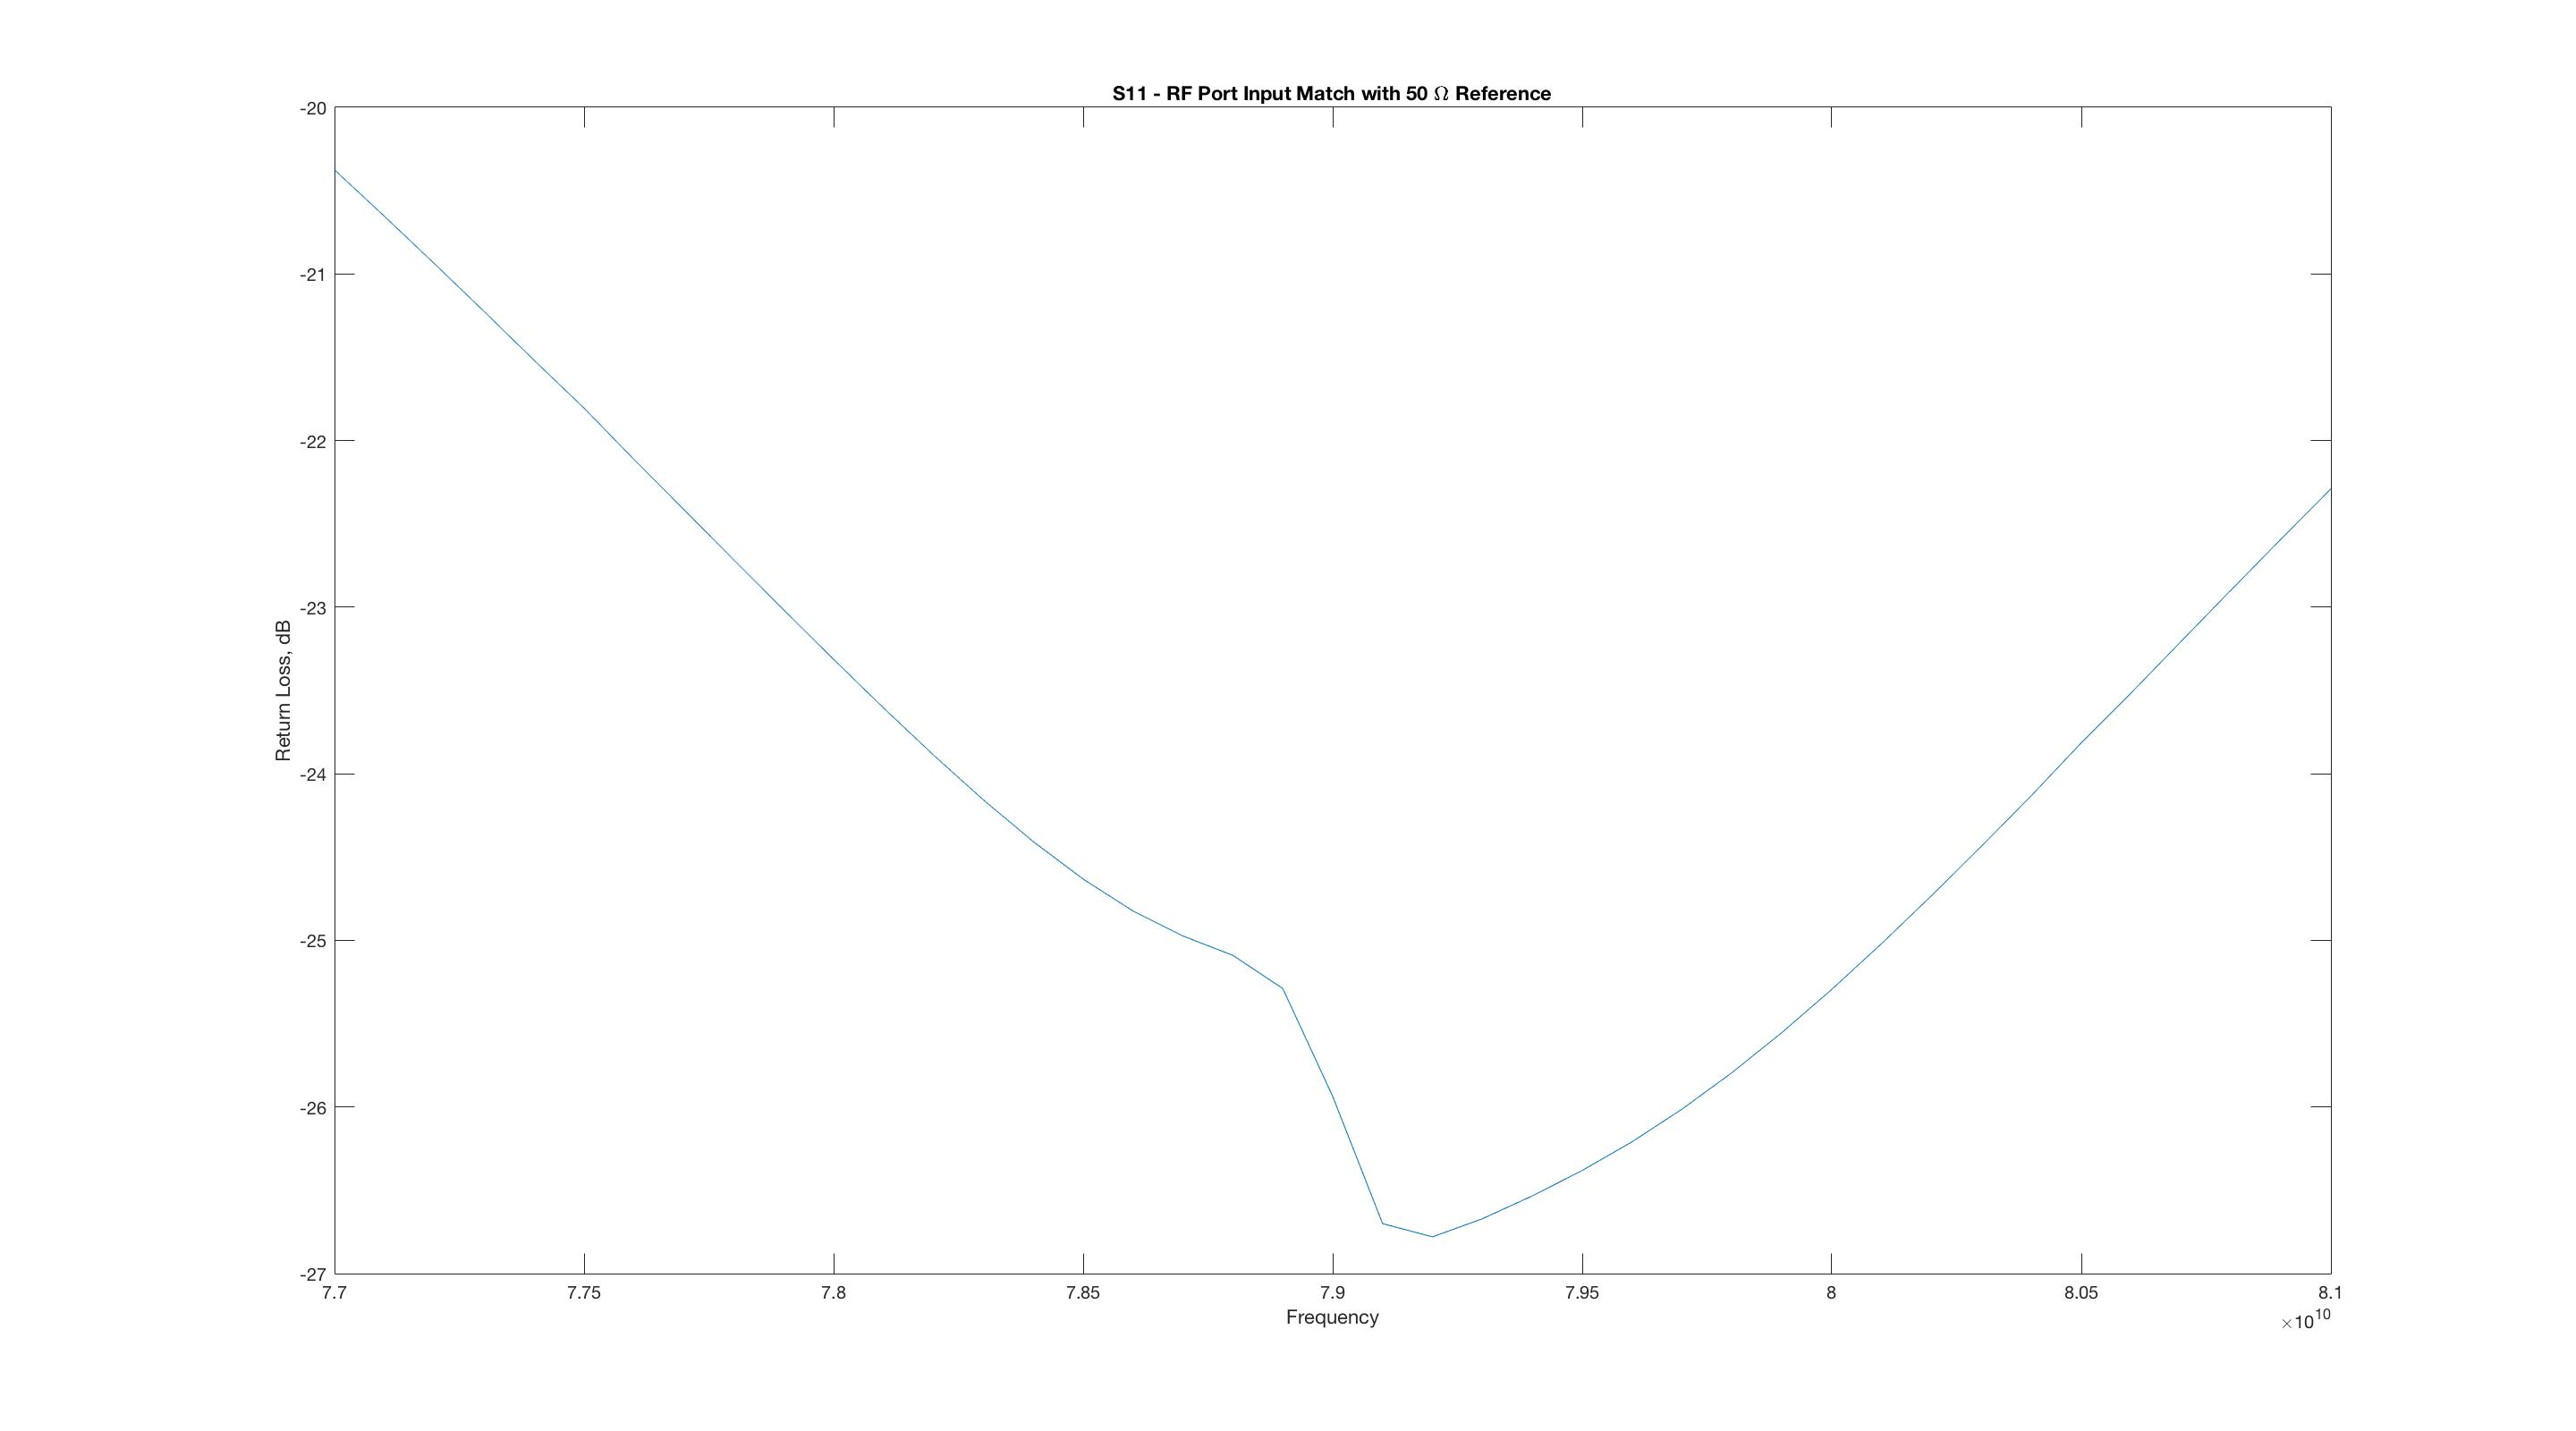
\includegraphics[width=0.95\textwidth] {Plots/S11.jpg}
  \caption{Final Return Loss of RF Port}
    \label{fig:matS11}
\end{figure}
\begin{figure}[H]
  \centering
  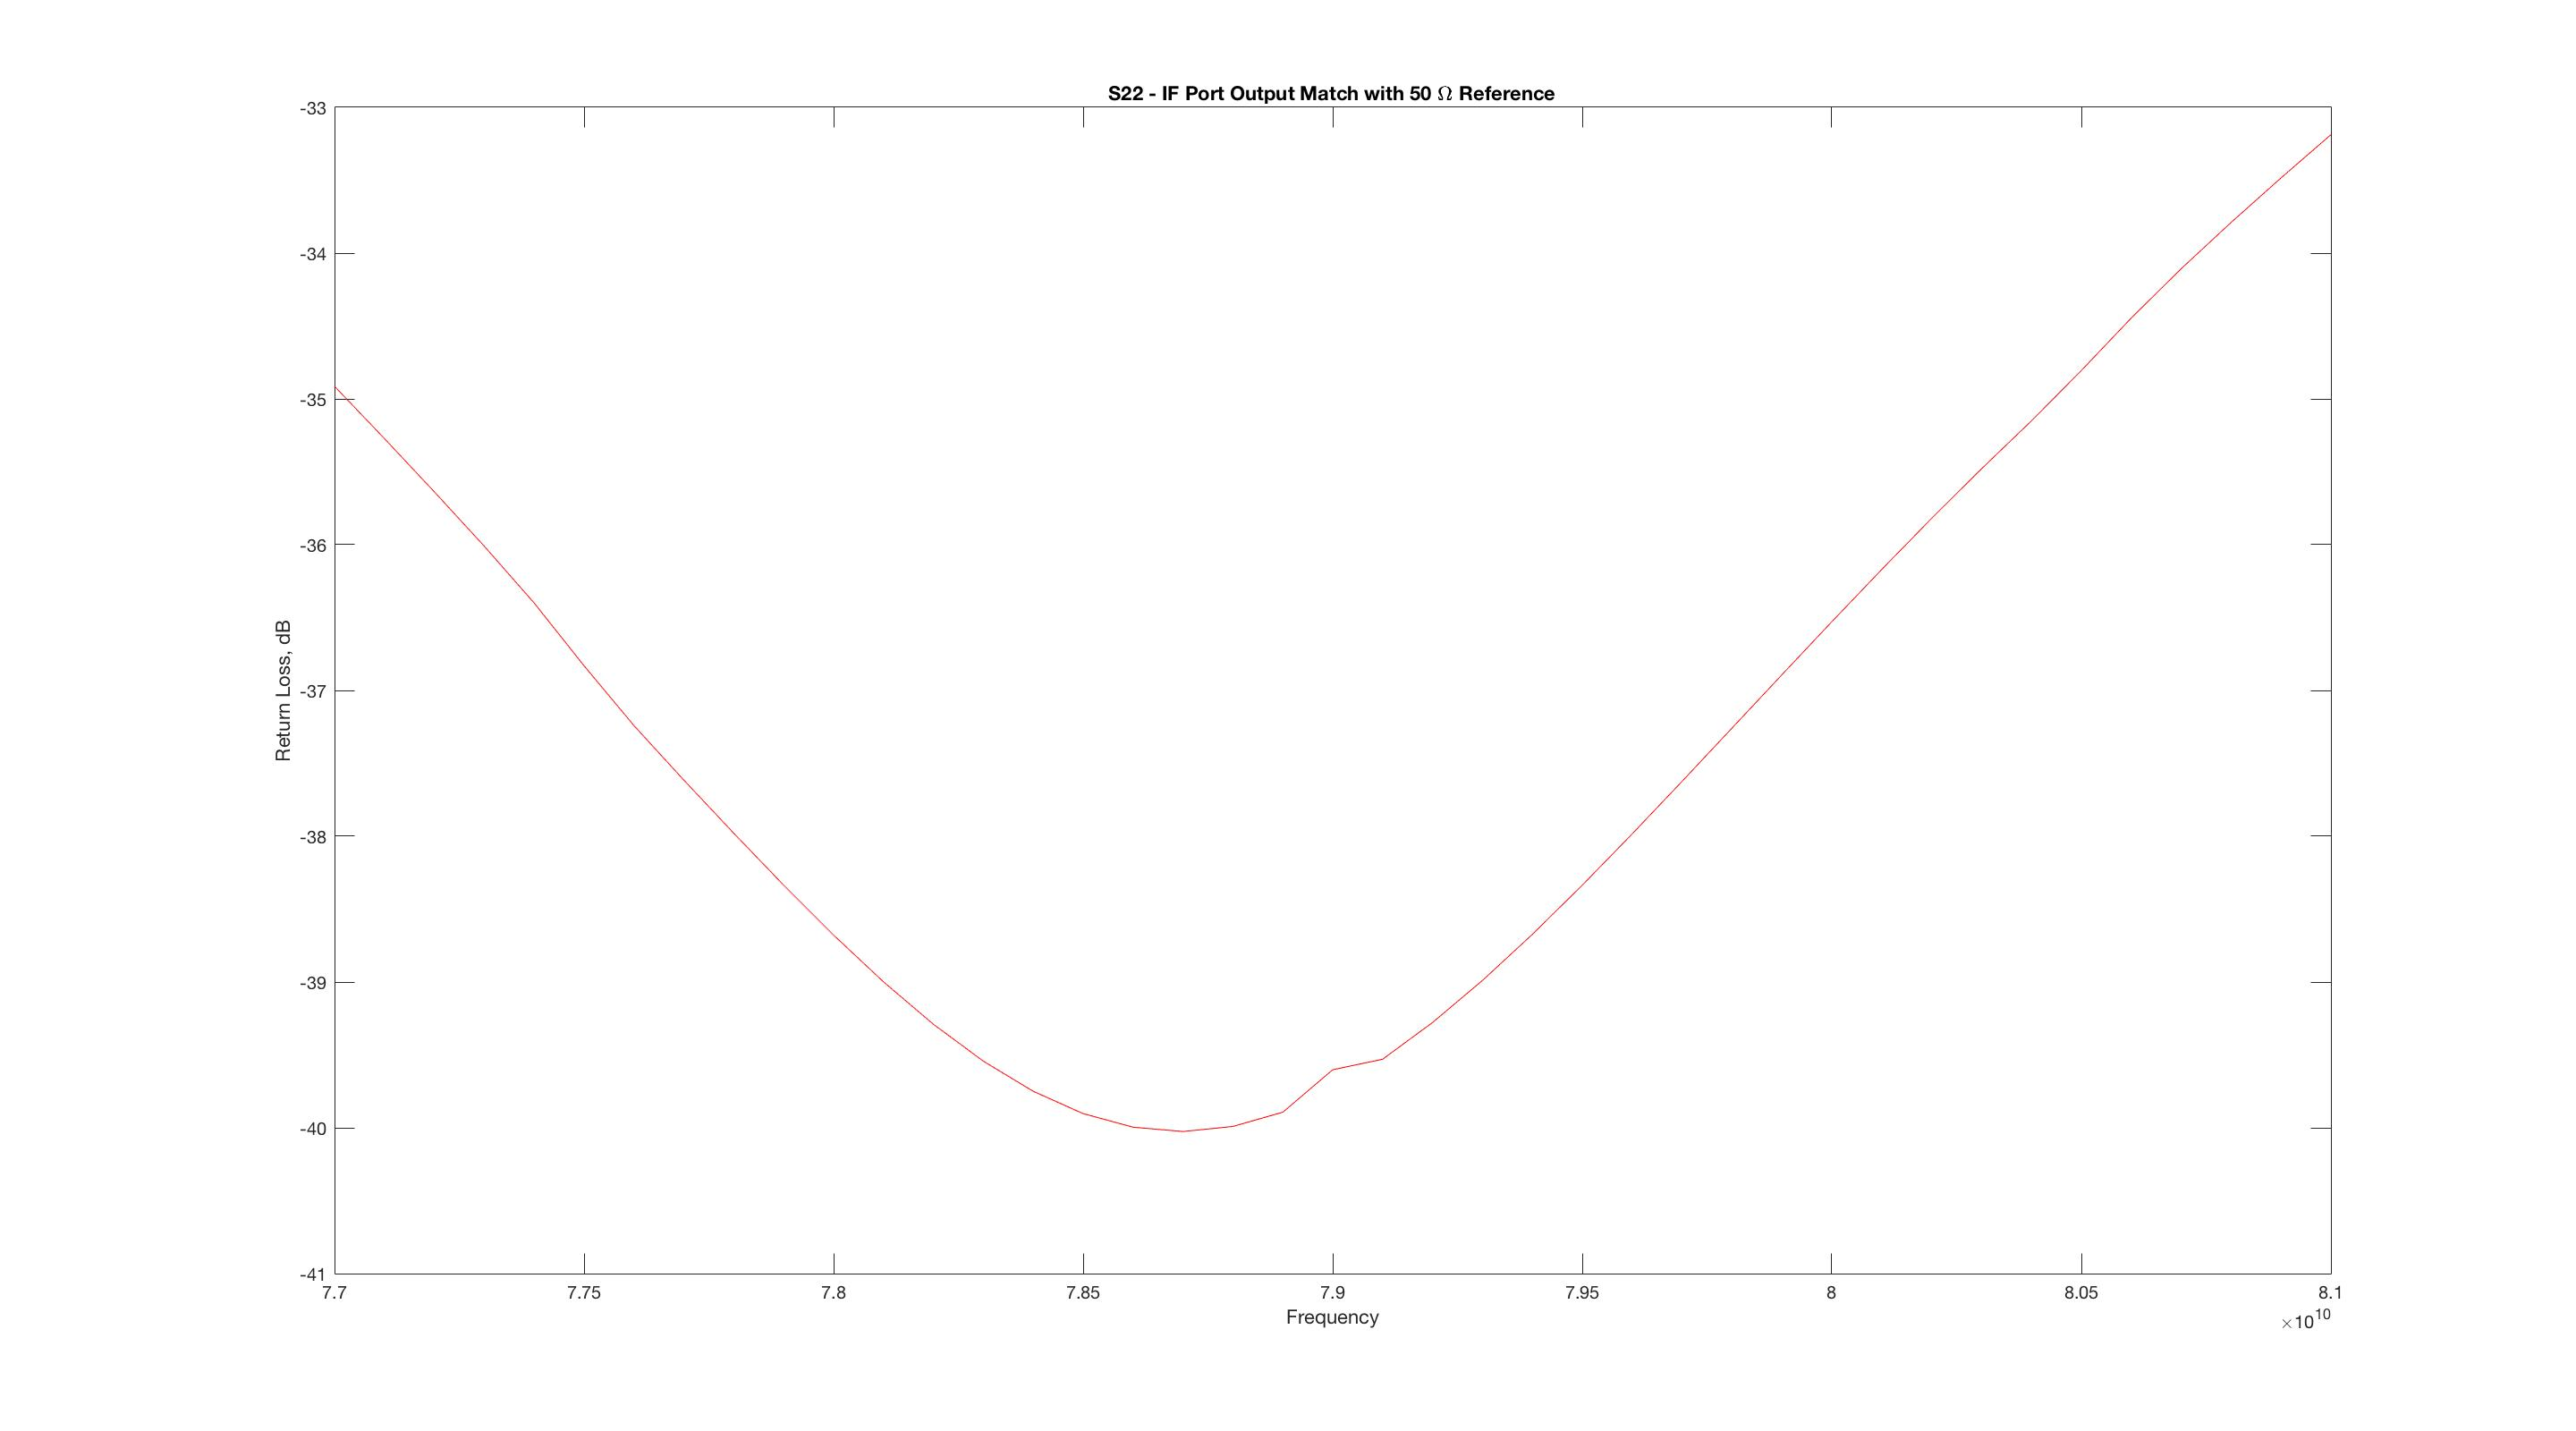
\includegraphics[width=0.95\textwidth] {Plots/S22.jpg}
  \caption{Final Return Loss of IF Port}
    \label{fig:matS22}
\end{figure}

The matching for the LO ports is simply done with two, $50 \Omega$ resistors. Simulations
showed almost infinitely small return loss as expected.
\subsection{Noise Figure}
\begin{figure}[H]
  \centering
  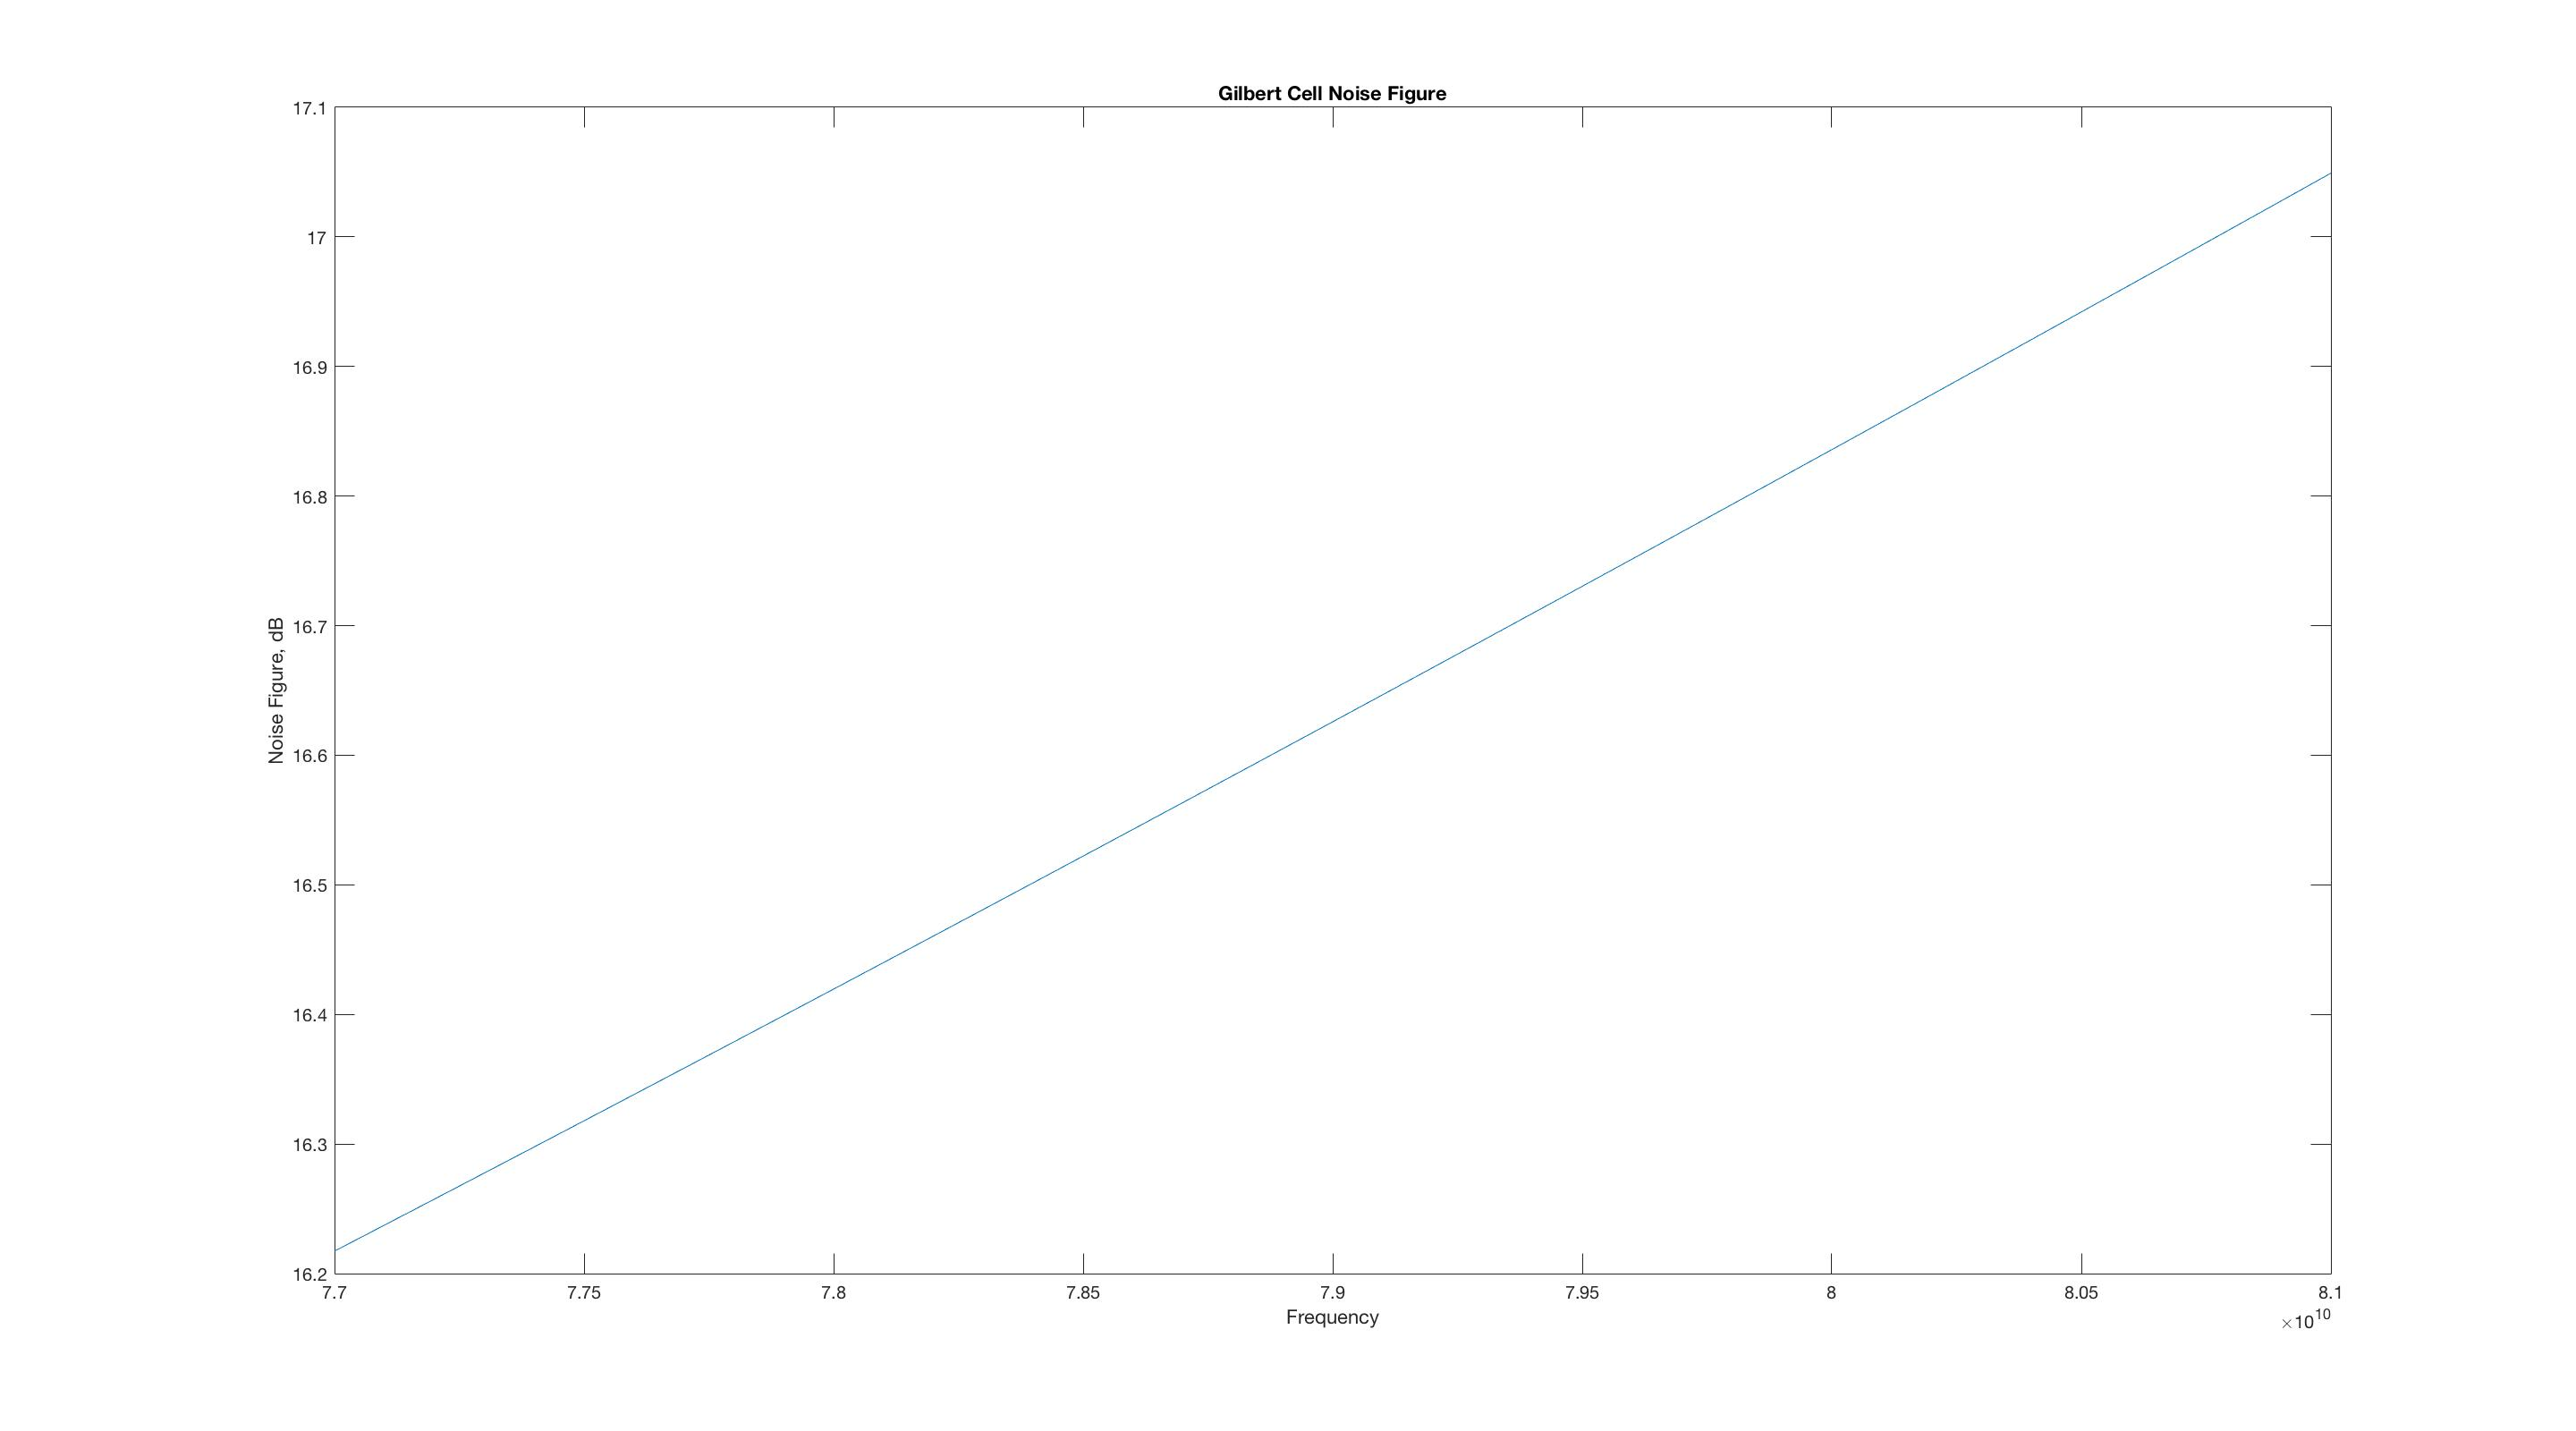
\includegraphics[width=0.95\textwidth] {Plots/NF.jpg}
  \caption{Final NF}
    \label{fig:matNF}
\end{figure}

\subsection{P1dB \& IP3}
The simulated values for P1dB and IP3 seem reasonable. The power is compressed at $\approx$
1dBm input and so this mixer could seemingly be used in the proposed implementation. Although
much further system analysis would obviously be required. The estimate of $IIP3 \approx P1dB+10dB $
seems to be relatively accurate.

\newpage
\section{Discussion \& Future Improvements }
The first goal of this project, which was to learn a lot, was certainly achieved. With regards to millimeter wave design it is clear that
many of the design techniques/equations used at lower frequencies will not be very accurate. Additional un-idealities such as inductor
Q and bulk modulation are not even taken into account in these simulations.
For example, many iterations of S-Parameter analysis
was required to get the circuit matched properly, particularly the output impedance which had values that were very different than initial  estimates.
It's apparent that the power budget would need to be increased to get reasonable gain. Furthermore, voltage headroom becomes an important consideration at
millimeter wave because of the small breakdown voltage.

%----------------------------------------------------------------------------------------
%	REFERENCES
%----------------------------------------------------------------------------------------
\section{References}
\printbibliography[heading=none]

\newpage
%----------------------------------------------------------------------------------------
%	APPENDIX
%---------------------------------------------------------------------------------------
\begin{appendices}
\section{Cadence Simulation Plots}\label{app:cresults}
\subsection{Conversion Gain}
\begin{figure}[H]
  \centering
  \includegraphics[width=0.95\textwidth] {Figures/FinalConversionGain.bmp}
  \caption{Conversion Gain Cadence}
    \label{fig:cGain}
\end{figure}
\subsection{RMS Spectrum}
\begin{figure}[H]
  \centering
  \includegraphics[width=0.95\textwidth] {Figures/FinalSpectrum.bmp}
  \caption{RMS Spectrum Cadence}
    \label{fig:cSpectrum}
\end{figure}
\subsection{Noise Figure}
\begin{figure}[H]
  \centering
  \includegraphics[width=0.95\textwidth] {Figures/FinalNF.bmp}
  \caption{Noise Figure Cadence}
    \label{fig:cNF}
\end{figure}
\subsection{P1dB}
\begin{figure}[H]
  \centering
  \includegraphics[width=0.95\textwidth] {Figures/P1dB_GOOD_ATTEMPT1_77point5.bmp}
  \caption{P1dB Cadence}
    \label{fig:cP1db}
\end{figure}
\subsection{IP3}
\begin{figure}[H]
  \centering
  \includegraphics[width=0.95\textwidth] {Figures/IP3dB_GOOD_ATTEMPT1.bmp}
  \caption{IP3 Cadence}
    \label{fig:cIP3}
\end{figure}
\subsection{S11}
\begin{figure}[H]
  \centering
  \includegraphics[width=0.95\textwidth] {Figures/FinalS11_rect.bmp}
  \caption{RF Port Match}
    \label{fig:cS11}
\end{figure}
\subsection{S22}
\begin{figure}[H]
  \centering
  \includegraphics[width=0.95\textwidth] {Figures/FinalS22Rect.bmp}
  \caption{IF Port Match}
    \label{fig:cS22}
\end{figure}

\newpage
\section{Improved Impedance Model}\label{app:imp}
\begin{figure}[H]
  \centering
  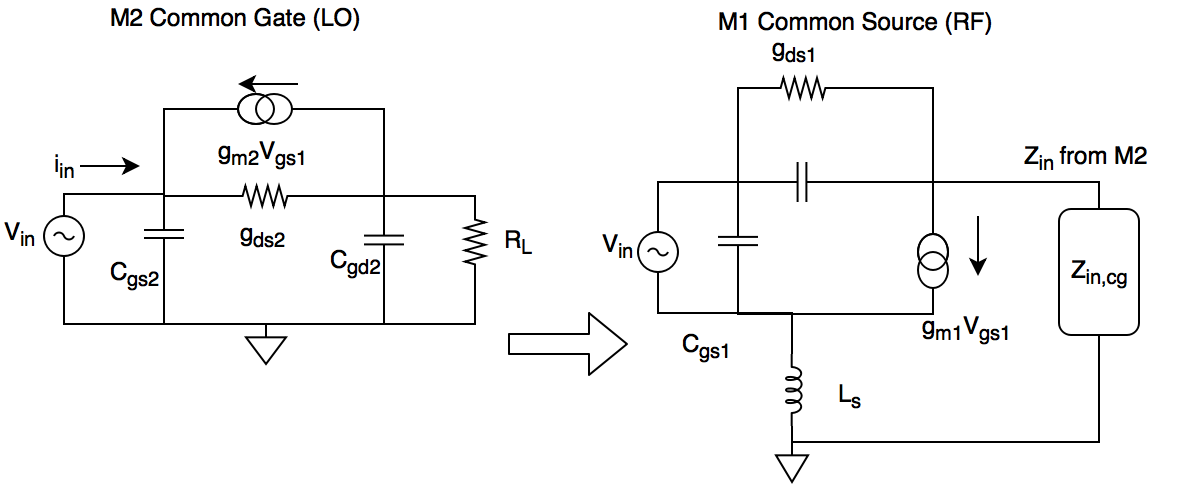
\includegraphics[width=0.65\textwidth] {Figures/smallsignal.png}
  \caption{Small Signal Models for Transistors}
    \label{fig:smallsig}
\end{figure}
First we take a look at the impedance looking into the common gate (LO) transistor. We'll call this
transistor M2 as seen in Figure

$$ i_{in} = V_{in}sC_{gs}+ g_mV_{in} +(V_{in}-V_{out})g_{ds} $$
@ $V_{out}$
$$V_{out}(sC_{gd}+g_L+g_{ds}) + V_{out}g_L + (V_{out}-V_{in})g_{ds} = g_mV_{in} $$
$$ Z_{in} = \dfrac{1}{sC_{gs}+g_m+g_{ds}-\dfrac{(g_m+g_{ds})g_{ds}}{g_{ds}+g_L+sC_{gd}}}$$
Now analyzing the impedance looking into the source degenerated common source (RF) transistor terminated
with the impedance of the common gate we just found.

$$i_in = (V_{in} - V_s)sC_{gs}+(V_{in}-V_{out})sC_{gd}+(V_{in}-V_{out})g_{ds}$$
@ $V_s$
$$ (V_s-V_{in})sC_{gs}+V_s/L_s = (V_{in}-V_s)g_m$$
$$ V_s = \dfrac{(sC_gs+g_m)V_{in}}{sC_{gs}+g_m+\dfrac{1}{sL_s}} = X\times V_{in}$$
@ $V_{out}$
$$ V_{out}(y_{in}) +g_mV_{in}-g_mXV_{in} +V_{out}sC_{gd}-V_{in}sC_{gd}+V_{out}(g_{ds})-V_{in}(g_{ds}) = 0$$
$$ V_{out} = \dfrac{(g_mX+sC_{gd}+g_{ds}-g_m)V_{in}}{y_{in}+sC_{gd}+g_{ds}}= Y\times V_{in}$$

\vspace{3mm}From here we can calculate the complete Input impedance looking into the RF port:
$$ Z_{in,total} = \dfrac{1}{ sC_{gs}-XsC_{gs}+sC_{gd}-YsC_{gd}+g_{ds}-Yg_{ds} } $$


\vspace{3mm}With a given value of $L_s$ in Matlab it was possible to calculate the Real and Img impedances
looking into the port. While this was an interesting exercise it did not prove to be any more accurate
than the simplified method. This is likely because of all the other parasitics that are still not taken into account.


\end{appendices}

\end{document}
